\documentclass[sigconf,anonymous,review]{acmart}
\usepackage{booktabs,array,tabularx}
\usepackage{algorithm,algpseudocode}
\algrenewcommand{\algorithmicrequire}{\textbf{Input:}}
\algrenewcommand{\algorithmicensure}{\textbf{Output:}}
\algrenewcommand{\algorithmicindent}{1.25em}
\algnewcommand{\algorithmicparallelfor}{\textbf{parallel for}}
\algdef{SE}[PAR]{ParallelFor}{EndParallelFor}[1]
  {\algorithmicparallelfor\ #1\ \algorithmicdo}{\algorithmicend\ \algorithmicfor}
\usepackage{tikz}
\usetikzlibrary{arrows.meta,positioning,calc}
\definecolor{inkblue}{RGB}{42,97,130}
\definecolor{mutedgreen}{RGB}{71,123,103}
\definecolor{mutedamber}{RGB}{173,124,52}
\definecolor{mutedred}{RGB}{153,77,82}
\newcolumntype{Y}{>{\raggedright\arraybackslash}X}
% System name macro: the preprint name is withheld for double-anonymous review.
\newcommand{\sys}{TreeHost}
\setcopyright{none}
\acmConference[ICPE '27]{18th ACM/SPEC International Conference on Performance Engineering}{May 24--28, 2027}{Gothenburg, Sweden}
\acmYear{2027}
\settopmatter{printacmref=false}
\acmISBN{}
\acmDOI{}
\begin{document}
\title{Hosting Tree Speculation on a Recurrent-Hybrid Model: Verifier Design, Audit Methodology, and Serving Evidence}
\author{Anonymous Author(s)}
\affiliation{\institution{Anonymous Institution}\country{}}
\begin{abstract}
Tree speculative decoding verifies many candidate continuations per step, but a recurrent-hybrid language model can host it only if every accepted path leaves consistent recurrent state, convolution history, and attention cache behind. We present \sys{}, a vLLM serving design in which a shared tree descriptor drives path-parallel recurrent verification, device-resident acceptance, and coordinated publication of the selected path into native running state. Because speculative serving on hybrid models has no settled measurement practice, we also contribute an audit methodology: a pooled completed-request decode-rate estimator with explicit exclusions, frozen recorded-request corpora with a disjoint-task generalization check, a frozen native-envelope numerical rule with planted state faults, a captured-row and Monte-Carlo sampler audit with planted faults, and an identical-prompt output-length comparability check. On Qwen3.8-27B NVFP4 on an NVIDIA DGX Spark, \sys{} verifies 27-candidate trees at 28.13 and 30.76 pooled tokens/s on two corpora, 7.7\% and 11.8\% above the same stack's five-token chain speculation and within 5\% of a tuned chain-speculation stack on a second serving system; 126 held-out continuation cycles stay within the frozen numerical bound while all ten planted faults are detected, and the deployed sampler shows no departure from the autoregressive target beyond a top-$k$ tie convention. A ten-task coding-agent study is reported descriptively. Tree verification is thereby available on a hybrid model at chain-stack cost; tree drafters are the untested next step.
\end{abstract}
\begin{CCSXML}
<ccs2012>
<concept><concept_id>10010147.10010178.10010179</concept_id><concept_desc>Computing methodologies~Natural language processing</concept_desc><concept_significance>300</concept_significance></concept>
<concept><concept_id>10011007.10010940.10010971.10011682</concept_id><concept_desc>Software and its engineering~Software performance</concept_desc><concept_significance>500</concept_significance></concept>
<concept><concept_id>10002944.10011122.10002945</concept_id><concept_desc>General and reference~Measurement</concept_desc><concept_significance>500</concept_significance></concept>
</ccs2012>
\end{CCSXML}
\ccsdesc[500]{Software and its engineering~Software performance}
\ccsdesc[500]{General and reference~Measurement}
\ccsdesc[300]{Computing methodologies~Natural language processing}
\keywords{speculative decoding, hybrid language models, Gated DeltaNet, LLM serving, measurement methodology, numerical reproducibility}
\maketitle

\section{Introduction}
Speculative decoding reduces serial target-model invocations by verifying draft tokens in parallel; its sampling guarantee assumes that verification supplies the intended target probabilities, and tree speculation widens the candidate set without relaxing that assumption~\cite{leviathan2023fast,chen2023sampling,miao2023specinfer}. Recurrent-hybrid models such as Qwen3-Next, which interleave Gated DeltaNet (GDN) layers with softmax attention, complicate the verifier: a candidate must inherit the recurrent state, convolution history, and attention cache of its ancestors, and the next serving iteration must inherit exactly the path selected for continuation~\cite{yang2024gated,wu2025stree}. A verifier can compute plausible candidate logits and still publish the wrong state.

This paper makes three contributions. \textit{First}, a verifier design that hosts 27-candidate trees on a hybrid model inside a production serving engine: branch paths are scanned in parallel from shared boundary states, acceptance runs on the device, and one accepted path is replayed into the native recurrent, convolution, and attention state through a shared logical-to-physical descriptor. A chain verifier cannot host tree drafters at all; this design is the substrate they need. \textit{Second}, a measurement and audit methodology for speculative serving on hybrid models, where decode rates, numerical agreement, and sampling correctness are each easy to mismeasure: a pooled completed-request decode-rate estimator with explicit exclusions; two frozen recorded-request corpora with a disjoint-task generalization check; a native-envelope numerical rule frozen before data collection, with ten planted state faults; a captured-row and Monte-Carlo audit of the acceptance walk with planted sampler faults; and an identical-prompt output-length comparability check. The methodology transfers to any speculative method on any hybrid model. \textit{Third}, evidence under that methodology on Qwen3.8-27B NVFP4 on an NVIDIA DGX Spark (GB10): \sys{} exceeds the same stack's five-token chain speculation by 7.7\% and 11.8\% pooled tokens/s on the two corpora and is within 5\% of a tuned chain-speculation stack on a second serving system, which measures the cost of hosting tree verification rather than a gain from it; 126 held-out continuation cycles satisfy the frozen numerical bound with every planted fault detected; the deployed sampler, audited on 2,480 captured rows, shows no departure from the autoregressive target beyond a top-$k$ tie convention. A ten-task SWE-bench Verified coding-agent study is reported descriptively.

The target workload is a long-running coding agent: generation alternates with repository inspection, tool execution, and tests, so performance depends on completed work as well as token production. We therefore report the model, serving route, task cohort, and measurement definition together, and we separate recorded-request replay, which fixes the prompts, from live agent runs, which do not. Section~\ref{sec:related} positions the design against the closest mechanisms; Section~\ref{sec:design} describes it; Section~\ref{sec:method} defines the methodology; Section~\ref{sec:results} reports the evidence; Section~\ref{sec:discussion} bounds it. Raw records, reducers, and the serving patches are in the anonymized artifact~\cite{anon2026artifact}.

\section{Background and Closest Designs}
\label{sec:related}
Speculative sampling constructs an exact target sample from proposal and residual distributions, conditional on the probabilities actually supplied~\cite{leviathan2023fast,chen2023sampling}. SpecInfer supplies the tree-verification framing; Sequoia, EAGLE-2, OPT-Tree, EAGLE-3, and DFlash study tree construction and drafters~\cite{miao2023specinfer,chen2024sequoia,li2024eagle,wang2024opt,li2025eagle3,chen2026dflash}; these drafting mechanisms are distinct from the verifier and state-publication choices studied here. PagedAttention and SGLang supply the scheduling and memory substrate, Marconi addresses prefix caching for hybrid models, and hybrid serving manages recurrent-state pools alongside KV storage~\cite{kwon2023efficient,zheng2024sglang,pan2024marconi,pytorch2025sglang,sglang2026qwen}. Flash-Decoding, FlashInfer, DeFT, and FastTree establish split-KV execution and tree-aware KV reuse~\cite{dao2023flashdecoding,ye2025flashinfer,yao2024deft,pan2025fasttree}; our modified FlashAttention-2 decode kernel applies grouped split-K execution under the tree's visibility and slot mapping~\cite{dao2023flashattention}.

Gated DeltaNet augments a decayed recurrent state with a data-dependent delta update~\cite{yang2024gated,yang2024delta}. Snakes and Ladders and STree use activation replay to recover state-space continuation state; SpecMamba and component-aware self-speculation study hybrid speculation further~\cite{wu2024snakes,wu2025stree,zhong2025specmamba,borobia2026component}. These works motivate an explicit state lineage; they do not make every recurrent update or numerical implementation interchangeable.

Six designs verify GDN trees or share recurrent state across candidates (Table~\ref{tab:related}). Weaver verifies with an ancestor-masked triangular solve and replays the selected path at commit time~\cite{oda2026marginals}; SpecLA keeps value tiles of recurrent state on chip within a chain, schedules ready chains in parallel, and buffers accepted factors for a later fused update~\cite{wang2026specla}; Bole evaluates a tree-structured finite-Neumann closed form, stores compact factors, reconstructs the accepted state, and integrates with SGLang~\cite{wang2026bole}; TreeWY solves a triangular system and fuses reconstruction of the previous accepted state with the next verification~\cite{ghantasala2026treewy,ghantasala2026treewycode}; ReplaySSM caches inputs and defers state materialization~\cite{replayssm2026}; OneLA shares a prompt-derived state across recommendation beams~\cite{yang2026onela}. Read-only verification followed by accepted-path replay and parallel chain scheduling are therefore direct prior art. \sys{} differs in continuation policy: it replays recorded operands through the serving engine's native per-layer GDN updates immediately after acceptance and publishes convolution and attention state through the same descriptor, so each iteration returns to the native state representation that prefix caching and serving graphs already use. Published speed ratios from different models and workloads are not combined into a ranking.

\begin{table}[t]
\caption{Recurrent verification and continuation policies. Mechanism comparison only; no performance ranking.}
\label{tab:related}
\centering\footnotesize
\begin{tabularx}{\columnwidth}{@{}>{\raggedright\arraybackslash}p{0.2\columnwidth}YY@{}}
\toprule
Method & Verification work & Continuation state \\
\midrule
Weaver~\cite{oda2026marginals} & Ancestor-masked triangular solve & Short selected-path recurrence \\
SpecLA~\cite{wang2026specla} & Resident state tiles; parallel chains & Buffered factors; later fused update \\
Bole~\cite{wang2026bole} & Finite-Neumann correction solve & Compact factors; state reconstruction \\
TreeWY~\cite{ghantasala2026treewycode} & Triangular solve in fused kernel & Prior-path reconstruction with next verify \\
ReplaySSM~\cite{replayssm2026} & Corrected inputs; cached transitions & Deferred state update \\
OneLA~\cite{yang2026onela} & Shared-base projections across beams & Compact per-beam transition records \\
\sys{} & Resident state tiles; parallel paths & Native replay; coordinated convolution and KV publication \\
\bottomrule
\end{tabularx}
\end{table}

\section{Verifier Design}
\label{sec:design}
\subsection{State boundary and shared descriptor}
Let $m$ be a materialized token prefix, the tokens already consumed by the target's forward computation, with persistent state $\mathcal{S}(m)=(R(m),C(m),K(m))$: recurrent matrices $R$, convolution histories $C$, and attention KV entries $K$. The logical emitted prefix may include a newly sampled token $b$ not yet consumed, so the continuation boundary is $(\mathcal{S}(m),b)$ rather than a claim that $\mathcal{S}(mb)$ exists. A tree descriptor holds candidate token IDs, parent indices, positions, attention visibility, and the map between logical nodes and physical slots. For one GDN head with state $R\in\mathbb{R}^{d_v\times d_k}$, decay $\alpha_i$, and write strength $\beta_i$, a node applies~\cite{yang2024gated}
\begin{align}
R'_i &= \alpha_i R_{\pi(i)}, & \delta_i &= \beta_i\bigl(v_i-R'_i k_i\bigr), & R_i &= R'_i+\delta_i k_i^\top, & o_i &= R_iq_i,
\end{align}
where $\pi(i)$ is the parent, which need not be the previous packed row. Causal convolution likewise needs path predecessors, and attention visibility must select the same logical ancestry; a correct attention mask cannot repair a wrong recurrent parent.

Figure~\ref{fig:pipeline} shows the cycle. Native multi-token prediction (MTP) supplies a principal chain and runner-up candidates; suffix prediction extends selected paths within a bounded capacity~\cite{oliaro2025suffix,arctic2026suffix,hu2024sam}. The verifier derives attention visibility, physical packing, path scheduling, and the acceptance walk from one logical topology; padding keeps execution shapes reusable while remaining invisible to attention and selection. The attention layout places the principal spine first in the physical suffix and applies the same permutation to KV write slots and ancestry-mask key columns, retaining logical query-row and position order; acceptance stays in logical-node space and publication maps selected nodes back to physical slots, so a layout optimization cannot silently change which entries a branch reads. Algorithm~\ref{alg:verify} states the contract: verification, selection, and publication all consume the same materialized path $A$, and a newly sampled token $b^*$ can be emitted while remaining pending. History-dependent logits processing (penalties) builds each verification row's history from its own root-to-node path (Section~\ref{sec:method-sampler}). Figure~\ref{fig:contract} summarizes the interface: all three state surfaces describe the same materialized prefix, and a pending token is created by the next forward.

\begin{figure}[t]
\centering
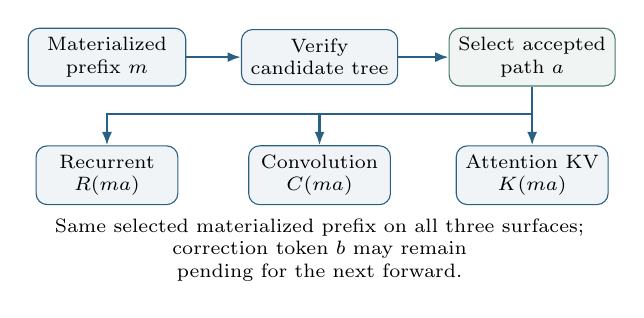
\begin{tikzpicture}[font=\scriptsize,
 box/.style={draw=inkblue,fill=inkblue!7,rounded corners,align=center,minimum height=0.7cm},
 arr/.style={-{Latex[length=1.7mm]},thick,draw=inkblue}]
\node[box,minimum width=2.0cm] (prefix) at (0,0) {Materialized\\prefix $m$};
\node[box,minimum width=1.8cm] (tree) at (2.7,0) {Verify\\candidate tree};
\node[box,draw=mutedgreen,fill=mutedgreen!8,minimum width=2.0cm] (path) at (5.4,0) {Select accepted\\path $a$};
\draw[arr] (prefix)--(tree);\draw[arr] (tree)--(path);
\node[box,minimum width=1.8cm] (r) at (0,-1.5) {Recurrent\\$R(ma)$};
\node[box,minimum width=1.8cm] (c) at (2.7,-1.5) {Convolution\\$C(ma)$};
\node[box,minimum width=1.8cm] (k) at (5.4,-1.5) {Attention KV\\$K(ma)$};
\draw[arr] (path.south) -- ++(0,-0.35) -| (r.north);
\draw[arr] (path.south) -- ++(0,-0.35) -| (c.north);
\draw[arr] (path.south)--(k.north);
\node[align=center,text width=7cm] at (2.7,-2.45) {Same selected materialized prefix on all three surfaces;\\correction token $b$ may remain pending for the next forward.};
\end{tikzpicture}

\caption{The accepted-prefix interface. Recurrent, convolution, and attention-KV state must all describe the same materialized prefix; a newly sampled correction or bonus token can remain pending until the next forward.}
\label{fig:contract}
\end{figure}

\begin{figure*}[t]
\centering
\resizebox{\textwidth}{!}{% Conceptual overview: the example path is selected after target verification.
% Recurrent replay, convolution gathering, and KV remapping are distinct operations.
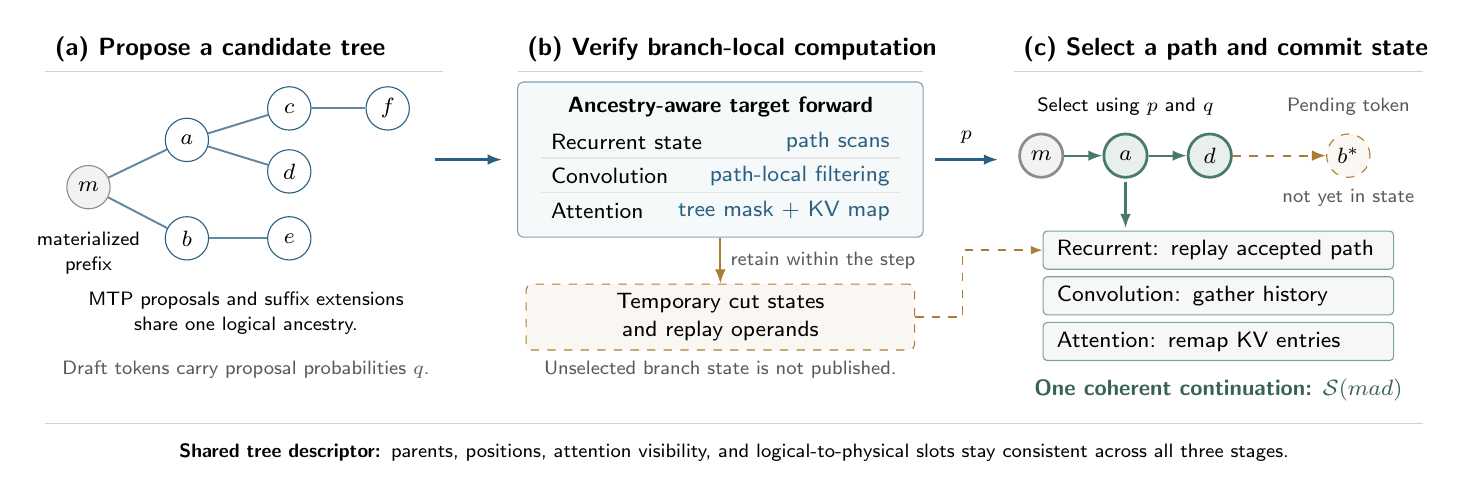
\begin{tikzpicture}[x=1cm,y=1cm,font=\sffamily\fontsize{8}{10}\selectfont,
  flow/.style={-{Latex[length=1.8mm]},draw=inkblue,line width=0.8pt},
  edge/.style={draw=inkblue!75,line width=0.7pt},
  token/.style={circle,draw=inkblue,fill=white,minimum size=5.5mm,inner sep=0pt},
  chosen/.style={token,draw=mutedgreen,fill=mutedgreen!12,line width=1pt},
  title/.style={anchor=west,font=\sffamily\bfseries\fontsize{9}{11}\selectfont},
  note/.style={font=\sffamily\fontsize{7.5}{9}\selectfont,align=center},
  state/.style={draw=mutedgreen!70,fill=mutedgreen!5,rounded corners=1.5pt,
    minimum height=0.37cm,text width=4.1cm,align=left,inner xsep=5pt}]

% Three stages, ordered by data flow.
\node[title] at (0,4.4) {(a) Propose a candidate tree};
\node[title] at (6.0,4.4) {(b) Verify branch-local computation};
\node[title] at (12.3,4.4) {(c) Select a path and commit state};
\draw[black!18] (0,4.12)--(5.05,4.12);
\draw[black!18] (6.0,4.12)--(11.15,4.12);
\draw[black!18] (12.3,4.12)--(17.5,4.12);

% An illustrative logical tree; no branch is accepted before verification.
\node[token,fill=black!5,draw=black!45] (root) at (0.55,2.65) {$m$};
\node[token] (a) at (1.8,3.25) {$a$};
\node[token] (b) at (1.8,2.0) {$b$};
\node[token] (c) at (3.1,3.65) {$c$};
\node[token] (d) at (3.1,2.85) {$d$};
\node[token] (e) at (3.1,2.0) {$e$};
\node[token] (f) at (4.35,3.65) {$f$};
\foreach \from/\to in {root/a,root/b,a/c,a/d,b/e,c/f}
  \draw[edge] (\from)--(\to);
\node[note,anchor=north] at (0.55,2.2) {materialized\\prefix};
\node[note,text width=4.7cm] at (2.55,1.05)
  {MTP proposals and suffix extensions\\share one logical ancestry.};
\node[note,text=black!65] at (2.55,0.33)
  {Draft tokens carry proposal probabilities $q$.};
\draw[flow] (4.95,3.0)--(5.8,3.0);

% This box denotes model components, not three independently executed models.
\node[draw=inkblue!60,fill=inkblue!4,rounded corners=2pt,
  minimum width=5.15cm,minimum height=1.97cm] (forward) at (8.575,3.0) {};
\node[font=\sffamily\bfseries\fontsize{8}{10}\selectfont] at (8.575,3.67)
  {Ancestry-aware target forward};
\node[anchor=west] at (6.3,3.23) {Recurrent state};
\node[anchor=east,text=inkblue] at (10.85,3.23) {path scans};
\node[anchor=west] at (6.3,2.79) {Convolution};
\node[anchor=east,text=inkblue] at (10.85,2.79) {path-local filtering};
\node[anchor=west] at (6.3,2.35) {Attention};
\node[anchor=east,text=inkblue] at (10.85,2.35) {tree mask + KV map};
\draw[black!10] (6.3,3.02)--(10.85,3.02);
\draw[black!10] (6.3,2.58)--(10.85,2.58);
\node[draw=mutedamber,fill=mutedamber!6,dashed,rounded corners=2pt,
  text width=4.7cm,align=center,minimum height=0.65cm] (scratch) at (8.575,1.0)
  {Temporary cut states and replay operands};
\draw[flow,draw=mutedamber] (forward.south)--(scratch.north)
  node[midway,right,note,text=black!65] {retain within the step};
\node[note,text=black!65] at (8.575,0.33)
  {Unselected branch state is not published.};
\draw[flow] (11.3,3.0)--(12.1,3.0)
  node[midway,above=2pt,note] {$p$};

% The selected branch need not be the principal drafting spine.
\node[chosen,fill=black!5,draw=black!45] (mout) at (12.65,3.05) {$m$};
\node[chosen] (aout) at (13.72,3.05) {$a$};
\node[chosen] (dout) at (14.79,3.05) {$d$};
\node[token,dashed,draw=mutedamber,fill=mutedamber!6] (pending) at (16.55,3.05) {$b^*$};
\draw[flow,draw=mutedgreen] (mout)--(aout);
\draw[flow,draw=mutedgreen] (aout)--(dout);
\draw[flow,dashed,draw=mutedamber] (dout)--(pending);
\node[note] at (13.72,3.67) {Select using $p$ and $q$};
\node[note,text=black!65] at (16.55,3.67) {Pending token};
\node[note,text=black!65] at (16.55,2.51) {not yet in state};
\node[state] (rcommit) at (14.9,1.85) {Recurrent: replay accepted path};
\node[state] (ccommit) at (14.9,1.27) {Convolution: gather history};
\node[state] (kcommit) at (14.9,0.69) {Attention: remap KV entries};
\draw[flow,draw=mutedgreen] (13.72,2.72)--(13.72,2.13);
\draw[-{Latex[length=1.5mm]},dashed,draw=mutedamber,line width=0.7pt]
  (scratch.east)--(11.65,1.0)--(11.65,1.85)--(rcommit.west);
\node[note,text=mutedgreen!80!black,font=\sffamily\bfseries\fontsize{8}{10}\selectfont]
  at (14.9,0.08) {One coherent continuation: $\mathcal{S}(mad)$};

% A common invariant, not another sequential pipeline operation.
\draw[black!18] (0,-0.35)--(17.5,-0.35);
\node[note,text width=17.2cm] at (8.75,-0.72)
  {\textbf{Shared tree descriptor:} parents, positions, attention visibility, and logical-to-physical slots stay consistent across all three stages.};
\end{tikzpicture}
}
\caption{Tree verification and accepted-path commitment. (a) Drafting provides a candidate tree and proposal probabilities $q$. (b) Branch-local computation produces target probabilities $p$ and retains temporary state. (c) Sampling selects a materialized path (here $a,d$); recurrent replay, convolution gathering, and KV remapping publish $\mathcal{S}(mad)$. The newly sampled token $b^*$ remains pending. One descriptor keeps logical ancestry and physical storage aligned.}
\label{fig:pipeline}
\end{figure*}

\begin{algorithm}[t]
\caption{Tree verification and native continuation}
\label{alg:verify}
\small
\begin{algorithmic}[1]
\Require Native continuation state; candidate tree $T$; proposal probabilities $q$
\Ensure Emitted tokens; updated native state; next drafter input; any pending token
\State Map $T$ to physical slots, positions, and ancestor masks.
\State $p\gets$ target probabilities from path-local GDN, convolution, and attention computation; retain candidate hidden states, rounded replay operands, convolution histories, and temporary KV entries.
\State $(A,b^*)\gets$ accepted materialized path and pending token from sampling with $p$ and $q$.
\For{each GDN layer}
  \State Replay recorded operands along $A$ into the native recurrent state; gather the convolution history for $A$ into the native running row.
\EndFor
\State Remap the accepted KV entries with the same logical-to-physical slot map; select the matching hidden-state row for the next drafter input.
\State Advance positions along $A$; keep $b^*$ pending until its target forward.
\end{algorithmic}
\end{algorithm}

\subsection{Path-parallel scan and accepted-path replay}
The GDN verifier decomposes the tree into dependent path groups, a scheduling family also used by SpecLA~\cite{wang2026specla}. A first path starts from the request's pre-tree state and exports the cut states that downstream paths need; a second level evaluates independent branch paths from those cut states. Each GPU program covers one path, head, and value tile and keeps the full key dimension in its working tile, so sequential updates reuse the tile through the path loop instead of loading a full recurrent state per node. Cut states and operand rings are temporary within a step; the durable continuation lives in the request-owned native running rows, and prefix-cache snapshots use that native layout. The two levels run as separate launches and exchange only boundary states. If a program exports $N_c$ cut states of value-tile width $B_v$ and key dimension $d_k$, their fp32 payload is $4N_cB_vd_k$ bytes; the reusable scratch allocation reserves a full slot per node, so allocated bytes differ from state traffic.

Verification uses sequential path scans with fp32 carried state, raw gate inputs, and in-kernel query/key normalization. Accepted-path replay uses the engine's native fused GDN update with the recorded accepted operands, one native call per layer in a captured graph, publishing in place to the fp32 state bank. Normalization, beta conversion, gate evaluation, and output casts can differ between the two implementations, so their finite-precision agreement is a measured property (Section~\ref{sec:res-component}), not a consequence of the shared real-arithmetic recurrence. Replay carries one state tile through a bounded path loop, $O(B_vd_k)$ in tree size; recorded operands and candidate outputs scale with the verification shape. Figure~\ref{fig:scan-replay} shows the state lifetime; Algorithm~\ref{alg:scan-replay} in Appendix~\ref{app:scan} gives the full procedure. Path decomposition caches state only where downstream paths branch and reuses it across independent work; recomputing ancestry would remove exports at the cost of repeated updates, and exporting every candidate state would trade more writes for less recomputation. The two-level schedule is one point in that space, and neither a shorter logical path nor fewer state writes alone establishes a faster complete request, which is why Section~\ref{sec:method} measures complete cycles.

\begin{figure}[t]
\centering
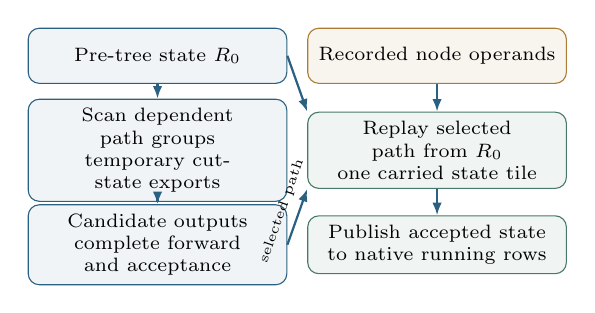
\begin{tikzpicture}[font=\scriptsize,
 box/.style={draw=inkblue,fill=inkblue!7,rounded corners,align=center,text width=3.05cm,minimum height=0.7cm},
 arr/.style={-{Latex[length=1.6mm]},thick,draw=inkblue}]
\node[box] (prior) at (0,0) {Pre-tree state $R_0$};
\node[box] (scan) at (0,-1.2) {Scan dependent path groups\\temporary cut-state exports};
\node[box] (out) at (0,-2.4) {Candidate outputs\\complete forward and acceptance};
\node[box,draw=mutedamber,fill=mutedamber!8] (ring) at (3.55,0) {Recorded node operands};
\node[box,draw=mutedgreen,fill=mutedgreen!8] (replay) at (3.55,-1.2) {Replay selected path from $R_0$\\one carried state tile};
\node[box,draw=mutedgreen,fill=mutedgreen!8] (publish) at (3.55,-2.4) {Publish accepted state\\to native running rows};
\draw[arr] (prior)--(scan);
\draw[arr] (scan)--(out);
\draw[arr] (ring)--(replay);
\draw[arr] (prior.east)--(replay.north west);
\draw[arr] (out.east)--node[above,sloped,font=\tiny]{selected path}(replay.south west);
\draw[arr] (replay)--(publish);
\end{tikzpicture}

\caption{State lifetime in the path-scan verifier. Temporary cut states connect path groups; recorded operands support selected-path replay. Only the accepted frontier becomes native persistent state.}
\label{fig:scan-replay}
\end{figure}

\subsection{Implementation changes around the verifier}
Three representations must agree: logical tree nodes, temporary verification storage, and the native state used by the next forward. Table~\ref{tab:optimization-map} lists the five implementation changes that carry one accepted path across them and the constraint that makes each nontrivial. \paragraph{One device-selected path drives continuation} Selecting output tokens does not update a hybrid model's state: the recurrent matrix must contain the accepted updates, convolution must retain the accepted history, attention must reference the accepted KV entries, and the drafter must receive the matching hidden row. Reconstructing these choices on the host inserts path-list preparation and synchronization between acceptance and publication. \sys{} instead emits fixed-shape device products (accepted node indices, path lengths, emitted tokens, the selected final row) that feed captured native replay, convolution gathering, KV remapping, and drafter-row selection. Recorded operands are staged for the native per-layer updates in one captured committer graph; emitted and materialized tokens stay distinct, and padded path entries never advance state. Serving, drafter, and committer stages are captured as separate graphs.

\paragraph{One slot map governs attention and publication} An ancestry mask specifies visible keys but not their physical placement or reduction groups; interleaving masked branch columns with spine keys changes the online-softmax reduction layout even when visibility is unchanged, which matters for finite-precision execution~\cite{he2025determinism}. \sys{} places the principal spine contiguously, applies the same permutation to KV write slots and mask key columns, keeps acceptance in logical-node space, and translates the selected nodes through that map at publication. The patched FlashAttention-2 decode kernel adds grouped query heads over shared staged KV tiles and split-K context partitions, established techniques~\cite{yao2024deft,pan2025fasttree} applied here under the tree's visibility and slot mapping; the component tests in Section~\ref{sec:res-component} measure its repeatability and reduction-order error, and the isolated effect of spine placement remains an ablation question.

\paragraph{Precomputed branch histories with preserved arithmetic} Static gather indices derived from the topology, windows gathered from the prior convolution history and candidate inputs, and fused ordered taps replace per-node history construction repeated across layers. Tap order and cast boundaries affect the values recorded for replay, and unused history positions must keep their padding, so the fused implementation retains the ordered operations and conversion points while replacing only the data movement; each layer still records and replays its own operands.

\paragraph{Fused draft selection that preserves proposals} At each MTP depth one full-vocabulary logits tensor serves the principal token and sibling candidates, and a fused kernel writes the spine token and three ordered candidate indices into reusable graph buffers. Reference argmax and top-$k$ do not share tie behavior, so taking the first top-$k$ result as the spine token would change the proposal tree; the fused selection preserves both reference outputs, including duplicate proposals where the reference produces them, and exact-output and captured-replay tests check it (Section~\ref{sec:res-component}).

\begin{table*}[t]
\caption{Implementation changes around the path verifier and the coordination or numerical constraint that makes each nontrivial. Workload rates measure their combined execution.}
\label{tab:optimization-map}
\centering\footnotesize
\renewcommand{\arraystretch}{1.1}
\begin{tabularx}{\textwidth}{@{}>{\raggedright\arraybackslash}p{0.23\textwidth}YY@{}}
\toprule
Starting work or constraint & \sys{} change & What must remain consistent \\
\midrule
Host path-list construction between acceptance and publication & Device-selected path feeds captured native replay, convolution, KV and drafter selection & All consumers select the same materialized prefix; pending and padded tokens do not advance state \\
Logical ancestry does not determine physical KV placement & Spine-contiguous slots with coordinated writes, mask columns and accepted-path remap & Logical query order, physical source slots and native destination positions agree \\
Per-node convolution histories and repeated layer preparation & Static ancestry gathers, fused ordered taps and per-layer operand buffers & Tap order, cast boundaries, history padding and layer identity \\
Separate score preparation and argmax/top-$k$ operations & One shared logits tensor and fused selection into graph buffers & Both reference tie conventions, candidate order and duplicate behavior \\
Repeated KV staging and limited decode parallelism & Grouped query heads and split-K in the patched tree-attention kernel & Tree visibility and slot mapping across partitions; characterized reduction error \\
\bottomrule
\end{tabularx}
\end{table*}

\section{Measurement and Audit Methodology}
\label{sec:method}
\subsection{Platform, arms, and workloads}
All experiments use Qwen3.8-27B on one NVIDIA DGX Spark (GB10) with a ModelOpt mixed-precision checkpoint: NVFP4 target MLP weights and vocabulary projection, FP8 attention projections, BF16 activations and KV storage, FP32 recurrent state, and the checkpoint's one-layer BF16 MTP module as the only drafter in every arm. Three serving arms share this checkpoint: \sys{} and native five-token chain MTP on the same vLLM build, and SGLang EAGLE on a separate stack that invokes the same MTP module. The evaluated tree has 27 draft candidates and one root padded to 32 verification rows: five MTP passes supply 15 candidates and suffix prediction adds a six-token principal tail and rescue branches of four and two, for a maximum depth of eleven. Attention groups query heads in pairs over four context partitions; the model has 48 GDN and 16 attention layers. Sampling is temperature 0.6, top-$p$ 0.95, top-$k$ 20, min-$p$ 0, presence penalty 1.0, with no per-request seed. Appendix~\ref{app:settings} lists the serving settings. Three workloads are used: (i) a live coding-agent study, Qwen Code 0.19.4 on ten explicitly identified SWE-bench Verified Astropy tasks~\cite{jimenez2024swe}, once per task and arm, with a 24,000-token response cap and a 9,000-second task budget, where the benchmark evaluator tests nonempty patches and empty patches count as unresolved; (ii) recorded-request replay on two frozen corpora; and (iii) full-model continuation and component diagnostics.

\subsection{Decode-rate estimator and replay corpora}
\label{sec:method-rate}
For completed request $r$, let $n_r$ be the output-token count, $\ell_r$ the end-to-end latency, and $f_r$ the time to first output. We report the pooled decode rate
\begin{equation}
 D_{\mathrm{pool}} = \frac{\sum_{r=1}^{R}(n_r-1)}{\sum_{r=1}^{R}(\ell_r-f_r)},
 \label{eq:pooled-decode}
\end{equation}
over the same completed requests, so that the numerator counts output intervals and the denominator excludes first-output latency and between-request agent or tool work. Pooling matched token and time totals across runs weights long requests by their duration; the estimator measures token production over accumulated request time, not aggregate wall-clock throughput, and a change in it is not a task-completion speedup. For the live study the counts come from server metric counters bracketing each arm, checked for continuity, resets, and outstanding requests at task boundaries; for replay they come from the client stream and server completion counts.

The first replay corpus holds 43 requests recorded from two Astropy task conversations (prompt lengths 23,024--68,557 tokens); each configuration receives the same saved messages and tool definitions sequentially with one active request, a 1,024-token response cap, and the sampling settings above, and generated tool calls are not executed. vLLM arms share image, tokenizer, chat template, prefix caching, chunked prefill, and a 131,072-token context. For the cross-stack comparison the complete input token sequence is captured from vLLM's tokenizer and passed as IDs to SGLang, so all 43 inputs are token-identical. The second, disjoint corpus selects 43 of 61 requests captured from native-MTP agent executions on four further tasks across five conversations, allocated proportionally and spaced through capture order, with its manifest frozen before any replay and no message overlap with the first corpus; SGLang uses its chat endpoint there, so inputs match as messages but not as serialized IDs. Replay timing starts at the first nonempty streamed delta (first streamed completion-count increase for SGLang's token-ID endpoint) and ends at stream completion. Each principal vLLM arm is replayed three times per corpus; an exploratory native MTP sweep over one, three, five, and seven draft tokens and SGLang step/capacity settings has unequal repetition.

\subsection{Numerical agreement rule and planted faults}
\label{sec:method-numeric}
Component tests compare the tree verifier and the native chain on synthetic operand sets with the deployed tree geometry (32 physical rows, 28 accepted publication paths, 48 recurrent instances per set) against a float64 recurrence, requiring both root-mean-square and maximum absolute error to satisfy $E_{\mathrm{tree}}\leq 1.10E_{\mathrm{native}}+2^{-24}M_{64}+2^{-149}$, where $M_{64}$ is the reference's corresponding magnitude; each block runs twice in two fresh processes, and planted controls (sibling substitution, swapped state rings, stale publication metadata, off-path poisoning, zero replay) must be rejected.

The full-model comparison replays harvested natural accepted paths over six fresh prefixes of 23,000--46,000 tokens from four task conversations disjoint from both replay corpora, in five fresh serving processes: a sequential reference $A$, an independent process $B$, a native cache-capacity control $V$ matched to the candidate's KV allocation, a native packed-GDN-kernel variant $P$, and \sys{}. Each prefix supplies three seven-cycle schedules (cold with a common starting-state import, a cache-priming repeat, and a cache-resumed case without import), 126 cycles in total including a final root-only cycle that consumes the last pending token; every candidate forward is checked against all 32 recorded tree-input rows. For state or logit surface $s$ at cycle $c$ the reference envelope is $R_s(c)=\max\{F_s,d_s(B,A;c),d_s(V,A;c),d_s(P,A;c)\}$, with state distance the maximum per-layer relative $L_2$ error (floor $F_s=0.02$) and next-token KL divergence (floor $0.15$ nats); the candidate must satisfy $d_s\le 2R_s$ on every surface and cycle, and a greedy mismatch is tolerated only when $A$'s top-two logit margin lies within the native controls' own logit spread. The rule and constants were calibrated on an earlier collection and frozen before the fresh prefixes were evaluated. Ten planted faults, five types on two prefixes each (omitted convolution gathering, omitted recurrent replay, incorrect KV remapping, stale root input, sibling-state publication), must each exceed the base case's bound on the designated surface; cache-resumed cases must start at least 90\% cached; one candidate case is repeated in-process. Appendix~\ref{app:fullmodel-protocol} details the protocol.

\subsection{Sampler audit}
\label{sec:method-sampler}
The sampling rule is exact only when the supplied probabilities are correct, which for history-dependent processing means that a target row's penalty history is the path through its parent and a leaf continuation row's history includes the leaf. The audit has two parts. A record-only runtime wrapper captures, for 40 tree steps on four requests, the token set whose logits the processors changed in each of 2,480 target and continuation rows, and compares it with the per-path history reconstructed from the tree's parent table and with the flattened chain history a chain combiner would build. Then the deployed acceptance walk, whose CPU floating-point oracle the CUDA path matches byte for byte, is sampled 200,000 times on each of six captured steps; emitted-token counts conditional on visiting a node are compared with the supplied row and, separately, with the autoregressive row reconstructed under the native tie-keeping top-$k$, using an approximate chi-square $G$-test with pooled rare bins, at least 2,000 visits per node, and a Bonferroni-adjusted per-step threshold of $10^{-3}$. Five planted faults (temperature applied twice, target rows shifted, fixed residual draw, unconditional acceptance, correlated random draws) establish sensitivity. Two known differences from single-row decoding remain outside the audit: the tree path ignores min-$p$, and its top-$k$ retains exactly $k$ tokens where native decoding keeps boundary ties.

\subsection{Output-length comparability}
\label{sec:method-length}
If two arms sample the same target distribution, identical prompts must yield the same output-length distribution. For each replay corpus we compare, request by request, the mean output length over three tree runs with the mean over three chain-MTP runs, and report totals, the number of requests on which the tree arm is longer, and response-cap hits. This check separates sampling effects from trajectory effects in the live agent study, where arms diverge after their first tool call. Table~\ref{tab:instruments} summarizes what each instrument can and cannot establish.

\begin{table*}[t]
\caption{The measurement and audit instruments, what each establishes, and what it leaves open.}
\label{tab:instruments}
\centering\footnotesize
\renewcommand{\arraystretch}{1.1}
\begin{tabularx}{\textwidth}{@{}>{\raggedright\arraybackslash}p{0.2\textwidth}YY@{}}
\toprule
Instrument & Establishes & Leaves open \\
\midrule
Pooled decode rate, Eq.~\ref{eq:pooled-decode}, on frozen replay corpora & Serving-rate differences between arms on identical requests, with run-to-run spread & Task-completion speed; endpoint and stack differences for SGLang; batch sizes above one \\
Disjoint-task corpus & Whether a difference tuned on one corpus reappears on unseen tasks & Statistical significance; one SGLang run; chat-level rather than token-level input parity \\
Component checks against a float64 recurrence & Verifier and committer error relative to the native chain on the deployed geometry, with planted controls & Behavior inside the full model; attention and convolution interplay \\
Frozen native-envelope rule with planted faults & Full-model continuation error within twice the native spread on every surface and cycle; detectability of five fault types & Bitwise or strict greedy equality; live acceptance loop; cache admission and eviction; 18 of all path combinations \\
Captured-row and Monte-Carlo sampler audit & Penalty histories on 2,480 rows; walk exactness on supplied rows; departure beyond the top-$k$ tie convention; fault sensitivity & Universal exactness; min-$p$; batch sizes above one \\
Identical-prompt output lengths & Whether two arms' length distributions agree on fixed prompts & Agent-trajectory divergence after the first tool call \\
Live coding-agent study & Outcomes, request counts, token volumes, and pooled rate per arm on ten named tasks & Benchmark-wide quality; isolated serving effects; trajectory variance with one attempt per arm \\
\bottomrule
\end{tabularx}
\end{table*}

\section{Results}
\label{sec:results}
\subsection{Recorded-request replay}
\label{sec:res-replay}
Table~\ref{tab:request-replay} reports complete configuration runs on the first corpus, each containing all 43 requests. Across three runs per arm, \sys{} records 28.13 pooled tokens/s and five-token native MTP records 26.12, a 7.7\% difference; individual run rates span 27.40--28.78 and 26.04--26.23 tokens/s. Plain autoregressive decoding records 10.54 tokens/s in one run, and five-token MTP has the highest pooled rate of the exploratory native sweep. SGLang EAGLE with seven steps and eight draft tokens, whose top-$k$ of one makes the draft a chain, yields 29.69 pooled tokens/s over three runs with identical incoming token IDs; attention, prefill settings, and endpoint timing still differ. Output-side counters pooled over the repeated vLLM runs give 4.35 accepted drafts per speculative event for \sys{} and 3.17 for five-token MTP; these counters describe emitted drafts, excluding the correction or bonus token. Exploratory variants that disable individual \sys{} optimizations, with their phase timers and drafting-pass sensitivity, are in Appendix~\ref{app:variants}; they predate the penalty-history correction and do not isolate single effects.

\begin{table}[t]
\caption{Sampled replay of 43 recorded requests, capped at 1,024 output tokens. Rates pool matched token and time totals across runs; ranges are individual run rates, not confidence intervals. SGLang receives the same input token IDs on a different stack and streaming endpoint.}
\label{tab:request-replay}
\centering\small
\begin{tabular}{@{}lrrr@{}}
\toprule
Configuration & Runs & Tokens/s & Run range \\
\midrule
vLLM autoregressive & 1 & 10.54 & --- \\
vLLM MTP, 1 token & 1 & 15.37 & --- \\
vLLM MTP, 3 tokens & 1 & 22.06 & --- \\
vLLM MTP, 5 tokens & 3 & 26.12 & 26.04--26.23 \\
vLLM MTP, 7 tokens & 1 & 25.72 & --- \\
\sys{} & 3 & 28.13 & 27.40--28.78 \\
\midrule
SGLang EAGLE, 7/8 & 3 & 29.69 & 28.91--30.90 \\
\bottomrule
\end{tabular}
\end{table}

\begin{table}[t]
\caption{Disjoint 43-request replay. Rates pool matched totals; ranges are individual run rates. Request messages are shared, but SGLang uses a different chat serialization.}
\label{tab:disjoint-replay}
\centering\small
\begin{tabular}{@{}lrrr@{}}
\toprule
Configuration & Runs & Tokens/s & Run range \\
\midrule
\sys{} & 3 & 30.76 & 30.38--31.14 \\
vLLM MTP, 5 tokens & 3 & 27.52 & 27.41--27.71 \\
SGLang EAGLE, 7/8 & 1 & 30.24 & --- \\
\bottomrule
\end{tabular}
\end{table}

On the disjoint corpus (Table~\ref{tab:disjoint-replay}), \sys{} records 30.76 pooled tokens/s against native MTP-5's 27.52, an 11.8\% difference, and every individual tree rate exceeds every MTP-5 rate. SGLang records 30.24 in its single run. The pooled tree--SGLang difference is within 5\% on both corpora and changes sign between them: \sys{} reaches a chain stack's rate while verifying 27-candidate trees, so that comparison measures the cost of hosting tree verification rather than a gain from it. The second corpus supports the direction of the MTP-5 difference without establishing statistical significance, equal output distributions, or task-completion improvement.


\subsection{Coding-agent study}
\label{sec:res-agent}
The coding-agent study completes 40 attempts, one per task and arm, with plain autoregressive decoding of the same checkpoint on the same vLLM build as the control (Table~\ref{tab:agent-study}; task-level outcomes in Appendix~\ref{app:workload}). \sys{} resolves five tasks with eight nonempty patches, of which three fail tests, and two empty patches; native MTP-5 resolves six with two failing and two empty; SGLang resolves five with three failing and two empty; plain decoding resolves seven with three failing and no empty patch. Empty patches count as failures without invoking the evaluator. The live trajectories diverge after the first tool call: \sys{} emits 258,889 output tokens over 248 requests, against 134,643 over 224 for MTP-5, 158,827 over 210 for SGLang, and 98,477 over 231 for plain decoding, so its lower pooled decode rate and longer summed agent duration here contrast with the fixed-request replays. The control decodes at 10.54 tokens/s, 2.5 times slower than \sys{}, yet its summed agent duration is shorter than \sys{}'s because it emits 2.6 times fewer tokens; all three speculative arms emitted more tokens than plain decoding. The replay check in Section~\ref{sec:res-sampler} finds no large aggregate length shift between the tree and chain arms on fixed prompts; with one attempt per arm, the live token-volume differences cannot be separated from trajectory variance, and their cause remains unresolved. The study is descriptive: one attempt per arm, ten selected tasks, and no benchmark-wide quality estimate.

\begin{table}[t]
\caption{Ten-task coding-agent study, one attempt per task and arm; plain decoding is the same-build control without speculation. Minutes sum agent durations, including tools but excluding server startup and evaluation. Decode rates use server-counter differences in Eq.~\ref{eq:pooled-decode}.}
\label{tab:agent-study}
\centering\small
\setlength{\tabcolsep}{3pt}
\begin{tabular}{@{}lrrrr@{}}
\toprule
Arm & Resolved & Requests & Tokens/s & Minutes \\
\midrule
\sys{} & 5/10 & 248 & 26.12 & 190.8 \\
Native MTP-5 & 6/10 & 224 & 27.17 & 99.5 \\
SGLang EAGLE & 5/10 & 210 & 29.89 & 103.0 \\
Plain decoding & 7/10 & 231 & 10.54 & 170.7 \\
\bottomrule
\end{tabular}
\end{table}


\subsection{Acceptance and execution spans}
\label{sec:res-spans}
The task study emits an average of 4.21 accepted drafts per \sys{} speculative event. This output-side counter excludes the correction or bonus token and does not identify the branch published into persistent state. Physical draft slots include padding and are distinct from logical candidates.

\begin{table}[t]
\caption{\sys{} acceptance and mean execution spans. Dispatch includes acceptance, path handling, and state commitment. GPU timers divide each duration sum by its own span count; wall time covers the decoding step. Disjoint replay pools three runs.}
\label{tab:recovered-telemetry}
\centering\small
\begin{tabular}{@{}lrr@{}}
\toprule
Metric & Task study & Disjoint replay \\
\midrule
Accepted drafts per event & 4.21 & 4.73 \\
Target GPU span (ms) & 115.43 & 109.84 \\
Drafter GPU span (ms) & 55.64 & 48.17 \\
Dispatch GPU span (ms) & 20.27 & 20.99 \\
Step wall time (ms) & 198.88 & 185.16 \\
\bottomrule
\end{tabular}
\end{table}

Table~\ref{tab:recovered-telemetry} characterizes the complete \sys{} cycle on these workloads. Dispatch combines sampling and native replay; the GPU spans do not form an isolated critical-path decomposition. Acceptance and phase durations vary with the request corpus, so higher replay acceptance is not evidence of better task quality.


\subsection{Component numerical checks}
\label{sec:res-component}
% Manuscript prose adapted from the generated component result; numerical data unchanged.
\begin{table}[t]
\centering
\caption{GDN component checks on GB10. Bitwise columns compare with the native chain; the paired rule compares both implementations with a float64 reference. Counts are per block and process.}
\label{tab:gdn-component}
\small
\setlength{\tabcolsep}{3pt}
\begin{tabular}{@{}lrrr@{}}
\toprule
Operand sets & \shortstack{BF16 output\\bitwise} & \shortstack{FP32 state\\bitwise} & \shortstack{Paired rule\\passed} \\
\midrule
Calibration & 3,004/3,072 & 2,688/2,688 & 5,760/5,760 \\
Held-out & 3,018/3,072 & 2,688/2,688 & 5,760/5,760 \\
\bottomrule
\end{tabular}
\end{table}

We test GDN verification and accepted recurrent-state publication on two calibration and two held-out synthetic operand sets. Each set supplies 48 recurrent instances with the evaluated tree geometry: 32 physical output rows, including padding, and 28 accepted publication paths. Each block runs twice in each of two fresh processes. These repetitions check reproducibility; they do not increase the number of distinct inputs.

For each head, we compare both implementations with a float64 recurrence. We require both root-mean-square and maximum absolute errors to satisfy
\begin{equation}
 E_{\mathrm{tree}} \leq 1.10 E_{\mathrm{native}} + 2^{-24} M_{64} + 2^{-149},
\end{equation}
where $M_{64}$ is the corresponding root-mean-square or maximum magnitude of the reference. Table~\ref{tab:gdn-component} reports all enumerated cases passing in both processes. All published recurrent states are bitwise equal to the native chain, while 68 calibration and 54 held-out output tensors differ in BF16 rounding. Native and candidate results reproduce bitwise across repeats and processes.

Calibration controls detect sibling substitution, swapped state rings, and stale publication metadata. Poisoning an off-path branch leaves the tested selected-path state unchanged, and a zero-replay control is rejected. These results support the tested GDN scan and recurrent publication mechanism.


The fused selection kernel records zero byte mismatches against the reference argmax and top-$k$ over 1,368 input cases and five block-count settings (6,840 configurations) and over 24 captured-graph replays; planted controls fire. The patched attention kernel gives bit-identical output and log-sum-exp across repeats in sixteen determinism cases with matching digests across two processes; on synthetic operands at model scales, 93.31\% of outputs agree with the reference within two ULP, the maximum output difference is $2^{-8}$, and log-sum-exp disagreement is at most four ULP, with all nine declared checks passing. Runtime traces confirm the specialized kernel in all sixteen attention layers, fused selection, device acceptance, and captured publication during the workload runs.

\subsection{Full-model continuation}
\label{sec:res-fullmodel}
All 126 cycles satisfy the frozen rule (Table~\ref{tab:fullmodel-agreement}), and all ten planted faults are detected at their mutation cycles, the weakest at 3.19 times its bound. The candidate greedy token matches $A$ on 121/126 cycles; the five disagreements occur where the reference's top two logits tie exactly. The separate-process, cache-capacity, and packed-kernel controls agree with $A$ on 125, 125, and 123 cycles. Every cache-resumed case starts with at least 91.9\% of its prefix cached across all five arms (30 observations), and the repeated candidate case is bitwise identical over its seven cycles. The result establishes agreement under the stated bounds, not bitwise model equality or strict greedy-output equality; harvested paths do not exercise the live acceptance loop, MTP drafter state, batch sizes above one, or cache admission and eviction.

\begin{table}[t]
\caption{Full-model continuation over 126 cycles. Maximum candidate error and candidate-to-native-envelope ratio may occur at different cycles; every ratio is below the frozen limit of 2. State errors are relative $L_2$; KL in nats.}
\label{tab:fullmodel-agreement}
\centering\small
\setlength{\tabcolsep}{4pt}
\begin{tabular}{@{}lrr@{}}
\toprule
Surface & Maximum error & Maximum ratio \\
\midrule
GDN recurrent state & 0.422 & 1.09 \\
Convolution history & 0.350 & 1.11 \\
KV, newly committed positions & 0.373 & 1.34 \\
KV, earlier positions & 0.248 & 1.07 \\
Next-token KL divergence & 0.095 & 0.63 \\
\bottomrule
\end{tabular}
\end{table}


\subsection{Sampler audit}
\label{sec:res-sampler}
All 2,480 captured rows carry the per-path penalty history; 82 coincide with the flattened chain history where the two agree. This capture postdates a correction: an earlier capture of the same deployment found all 2,480 rows flattened, with node-level total variation above 0.01 on about 22\% of deeper decisions (maximum 0.421), which the audit exposed and the serving patch repaired; every measurement in this paper uses the corrected sampler except the exploratory variants in Appendix~\ref{app:variants}. The Monte-Carlo test detects no departure in 48 node tests against the supplied rows. Against autoregressive rows reconstructed with the native tie-keeping top-$k$, one of 48 node tests rejects; across all 1,120 node-steps the reconstructed total variation is at most 0.028, and the three nodes above 0.01, including the rejected one, are exact ties at the top-$k$ boundary. All five planted fault types are detected in at least one of six steps (Table~\ref{tab:sampling-faults}). Non-rejection supports this finite check and does not prove universal exactness.

\begin{table}[t]
\caption{Sampler-audit fault sensitivity on six captured steps. Detection depends on which nodes the walk visits.}
\label{tab:sampling-faults}
\centering\small
\begin{tabular}{@{}lr@{}}
\toprule
Injected fault & Steps detected \\
\midrule
Temperature applied twice & 5/6 \\
Target rows shifted & 6/6 \\
Fixed residual draw & 4/6 \\
Unconditional acceptance & 3/6 \\
Correlated random draws & 1/6 \\
\bottomrule
\end{tabular}
\end{table}

The output-length check agrees: on identical prompts the corrected tree arm and MTP-5 produce 18,916 versus 18,504 mean output tokens over three runs on the first corpus and 15,270 versus 15,453 on the disjoint corpus, with the tree arm longer on 23 and 19 of 43 requests and similar response-cap counts. The live agent study's token gap therefore arises from diverging trajectories, not from sampling on a fixed prompt. An earlier ten-boot output-distribution diagnostic failed its frozen sensitivity requirement and is uninformative; the tree sampler seeds one process-wide generator with zero, so repeated boots with identical request order are not independent sampling replicates.


\section{Discussion and Threats to Validity}
\label{sec:discussion}
\subsection{Interpretation}
The design couples tree geometry, physical layout, and continuation publication: optimizing any one in isolation moves work elsewhere or invalidates another stage's mapping, and native replay pays accepted-path update work to return persistent state to the serving representation each iteration. The evidence supports three statements and no more. \sys{} exceeds the same stack's chain speculation by 7.7\% and 11.8\% pooled tokens/s on two corpora of fixed requests, and reaches a tuned chain stack's rate on a second serving system while verifying 27-candidate trees; tree drafters, which chain verification cannot host, are not evaluated. The implemented verifier and committer agree with native decoding within a frozen envelope that every planted state fault violates, and the deployed sampler shows no departure from the autoregressive target beyond the top-$k$ tie convention on the audited rows. The coding-agent study is descriptive: arms execute different request and tool trajectories, one attempt per arm cannot separate serving effects from trajectory variance, and identical-prompt output lengths show the token gap is not a sampling effect.

\subsection{Threats to validity}
\paragraph{External} Measurements use one model, one quantization, one GPU, and batch size one; equal memory-fraction settings do not equalize KV capacity, and boot allocation logs are not peak-memory measurements. \paragraph{Internal} Each principal vLLM arm has three replay repetitions, SGLang has one run on the disjoint corpus, and repeated tree boots reuse a process-seeded random sequence, so none of the differences carries a significance claim or a parity claim. \paragraph{Construct} The pooled estimator weights long requests by duration, subtracting one token approximates the first output interval, stream parsing remains inside the measured duration, and exact token-ID parity holds only for the first corpus's SGLang comparison. The numerical rule permits native-relative error and margin-bounded greedy disagreement rather than bitwise equality; 18 schedules do not exhaust path combinations. The sampler audit covers 2,480 captured rows and six Monte-Carlo steps; the ignored min-$p$ and the exact-$k$ top-$k$ convention are known, unaudited differences. The exploratory variant measurements in Appendix~\ref{app:variants} isolate only the split-K attention effect, and the isolated GDN kernel comparisons in Appendix~\ref{app:recurrent} use distinct numerical conventions and establish no accuracy ranking.

\section{Conclusion}
\sys{} hosts tree speculative verification on a recurrent-hybrid model inside a production engine by scanning paths in parallel and replaying one accepted path into native state through a shared descriptor. Under a frozen measurement and audit methodology, it verifies 27-candidate trees at 28.13 and 30.76 pooled tokens/s on two recorded corpora, 7.7\% and 11.8\% above same-stack chain speculation and within 5\% of a tuned chain stack, with 126 held-out continuation cycles inside the numerical bound, all ten planted faults detected, and a sampler audited on captured rows. Tree verification is thereby available on a hybrid model at chain-stack cost; the methodology is reusable for the tree drafters that should follow.

\bibliographystyle{ACM-Reference-Format}
\bibliography{ref}

\appendix
\section{Serving Configuration and Measurement Notes}
\label{app:settings}
\begin{table}[!htbp]
\caption{Serving settings for the task study. Native MTP, plain decoding, and \sys{} share the vLLM build. Exact versions and launch settings accompany the supplement.}
\label{tab:serving-config}
\centering\footnotesize
\renewcommand{\arraystretch}{1.12}
\begin{tabularx}{\columnwidth}{@{}>{\raggedright\arraybackslash}p{0.22\columnwidth}Y@{}}
\toprule
Setting & Configuration \\
\midrule
Target & Qwen3.8-27B; mixed NVFP4/FP8 weights, BF16 execution \\
Drafter & Same-checkpoint one-layer BF16 MTP in all arms; no separate EAGLE draft weights \\
\sys{} proposals & 27 drafts plus root, padded to 32 rows; maximum depth 11; five MTP passes and suffix extension \\
Native proposals & MTP: five drafts; plain decoding: none; SGLang: seven steps, top-$k$ one, capacity eight drafts \\
Attention & vLLM: forked FlashAttention-2; \sys{} adds grouping 2 and split-K 4; SGLang: FlashInfer \\
Scheduling & One active sequence; 4,096 prefill tokens for vLLM, 8,192 for SGLang \\
Context / memory & 131,072 tokens; memory fraction 0.70; actual KV capacities not equalized \\
Agent / budget & Qwen Code 0.19.4; one task at a time; 9,000 seconds \\
Response cap & 24,000 tokens per request \\
Sampling & Temperature 0.6; top-$p$ 0.95; top-$k$ 20; min-$p$ 0; presence penalty 1.0 \\
\bottomrule
\end{tabularx}
\end{table}

All tree runs use presence penalty 1.0. Tables~\ref{tab:agent-study}, \ref{tab:request-replay}, \ref{tab:disjoint-replay}, \ref{tab:recovered-telemetry}, \ref{tab:fullmodel-agreement}, and~\ref{tab:swe-tasks} use per-path penalty histories (Section~\ref{sec:res-sampler}); Tables~\ref{tab:replay-variants}--\ref{tab:drafting-passes} predate that correction. The exact-$k$ top-$k$ convention and ignored min-$p$ remain the differences from single-row decoding.

Workload rates use Eq.~\ref{eq:pooled-decode}; token counts and latency sums cover the same completed requests. First-output latency, tools, and evaluator time remain distinct from decode duration. GPU phase times divide each timer's duration sum by its own span count. Output-side acceptance counters describe emitted draft lengths and do not identify the committed tree path. For target probabilities $p$ and proposal probabilities $q$, rejection sampling combines accepted mass $\min(p,q)$ with residual mass proportional to $(p-q)_+$, which gives the target marginal for the probabilities actually supplied~\cite{leviathan2023fast,chen2023sampling}; serving additionally requires that subsequent forwards consume the state of the accepted path and that logits processing constructs that path's target distribution. The artifact~\cite{anon2026artifact} holds the serving patches, captured rows, reducers, and every record behind the tables.

\section{Task-Level Outcomes}
\label{app:workload}
Table~\ref{tab:swe-tasks} retains every attempt in the four-arm task study; the plain-decoding column is the same-build control without speculation; the \sys{} column is the attempt with the corrected sampler; the earlier pre-correction attempt is preserved in the supplement. Agent duration includes model service and tool execution, excluding server startup and subsequent evaluation. Empty-patch outcomes are distinguished from patches that reach the test evaluator.

\begin{table}[!htbp]
\caption{Task-level outcomes. IDs have prefix \texttt{astropy\_\_astropy-}. Each cell gives rounded agent minutes and outcome: R, resolved; F, failed tests; E, empty patch.}
\label{tab:swe-tasks}
\centering\small
\begin{tabular}{@{}lcccc@{}}
\toprule
Task suffix & \sys{} & MTP-5 & SGLang & Plain \\
\midrule
13977 & 11 / E & 10 / F & 21 / F & 13 / F \\
14096 & 18 / R & 20 / E & 10 / E & 33 / R \\
14182 & 24 / R & 6 / E & 1 / E & 11 / R \\
14309 & 11 / R & 2 / R & 2 / R & 4 / R \\
14365 & 10 / F & 2 / R & 3 / R & 8 / F \\
14369 & 25 / F & 18 / R & 16 / F & 29 / R \\
14508 & 38 / R & 7 / R & 7 / R & 12 / R \\
14539 & 6 / E & 3 / R & 17 / R & 20 / R \\
14598 & 37 / F & 27 / F & 20 / F & 29 / F \\
14995 & 11 / R & 5 / R & 5 / R & 12 / R \\
\bottomrule
\end{tabular}
\end{table}


\section{Full-Model Comparison Protocol}
\label{app:fullmodel-protocol}
The continuation comparison uses five fresh serving processes: sequential reference $A$, an independent process $B$, a native cache-capacity control $V$, a native packed-GDN-kernel variant $P$, and \sys{}. The reference uses a 40\,GiB KV allocation; $V$ uses the candidate's observed allocation. Candidate capacity follows its deployed memory-fraction policy. All arms consume matching forced tokens and positions and retain their own published state across subsequent cycles.

Six prefixes from four additional Astropy task conversations are disjoint from the earlier continuation and first replay corpora. A separate harvest records natural tree inputs and accepted paths. Each prefix supplies three seven-cycle schedules: a cold salted prefix with a common starting-state import, an unsalted repeat that primes the cache with the same import, and a cache-resumed case with no import. The last cycle accepts only the root to consume the final pending token; next-forward logits also observe the subsequent pending token. The root-only cycle is included in the 126-cycle total. Candidate-input checks compare every one of the 32 verification rows with the recorded tree.

The frozen numerical rule uses the largest same-cycle native-control distance, floored at 0.02 for state relative $L_2$ and 0.15 nats for next-token KL. Candidate distance must not exceed twice this envelope. A greedy mismatch is permitted only when $A$'s top-two logit margin is within $\max(0.25,2\max_{B,V,P}\|\Delta\mathrm{logit}\|_\infty)$ or the native controls are categorically unstable outside that band; at most 10\% of cells may be native-unstable. Input parity, complete sealed observations, starting-state read-back, and detection of every injected fault are prerequisites. These allowances make the verdict a numerical agreement test, rather than exact token or logit equality.

Five fault types run on two prefixes each at a selected natural cycle: omitted convolution gathering, omitted recurrent replay, incorrect KV remapping, stale root input, and sibling-state publication. Each must exceed the same base case's bound on its designated surface; sibling publication may exceed any of its three targeted state surfaces. Faults are reported separately from the 126 clean cycles. Prefix-cache coverage requires at least 90\% cached tokens in every cache-resumed observation. One clean candidate case is repeated in the same process. Earlier invalid forcing and insensitive comparison records remain in the supplement with their original dispositions.


\section{Path-Parallel Scan and Replay Procedure}
\label{app:scan}
\begin{algorithm}[h]
\caption{Path-parallel scan and accepted-path replay}
\label{alg:scan-replay}
\small
\begin{algorithmic}[1]
\Require Candidate tree $T$ and the pre-tree recurrent state for each GDN layer
\Ensure Recurrent outputs for all candidates; native recurrent state for the accepted path
\For{each GDN layer reached during the target forward}
  \State Compute and record this layer's rounded node operands.
  \For{each path group, in dependency order}
    \ParallelFor{each ready path, head, and value tile}
      \State Load the working state tile from the pre-tree state or a saved parent cut state.
      \For{each node on this path, in ancestry order}
        \State Update the working tile with this node's operands; write its recurrent output.
        \State Save the tile if a downstream path needs this node's state.
      \EndFor
    \EndParallelFor
  \EndFor
\EndFor
\State Complete the target forward and sampling to obtain the accepted materialized path $A$.
\For{each GDN layer}
  \State Start from this layer's pre-tree recurrent state.
  \For{each node on $A$, in path order}
    \State Apply the native GDN update using this layer's recorded operands.
  \EndFor
  \State Publish the resulting recurrent state to the request's native running row.
\EndFor
\end{algorithmic}
\end{algorithm}

\section{Exploratory Replay Variants}
\label{app:variants}
These measurements predate the penalty-history correction of Section~\ref{sec:method-sampler} and compare configurations under one sampler; they do not isolate single optimization effects.
Additional runs on the first corpus disable individual \sys{} optimizations (Table~\ref{tab:replay-variants}). The stock-attention variant completes all 43 requests in three runs and records 26.82 pooled tokens/s, 6.5\% below the deployed configuration measured under the same sampler; disabling fused draft selection or precomputed tap-operand preparation records 29.40 and 29.02 in one run each, within the deployed configuration's run-to-run spread. Phase timers (Table~\ref{tab:optimization-spans}) show the stock-attention variant with a 14.6\,ms longer target span and a 15.1\,ms longer step than two instrumented deployed repeats; fused selection off adds 0.7\,ms to the drafter span; operand-preparation removal has no clear separation. Boot logs report 20.54\,GiB of model-loading allocation in every variant and CUDA-graph pools of 1.52--1.59\,GiB (deployed), 0.42--0.50\,GiB (stock attention), 1.97\,GiB (fused selection off), and 1.47\,GiB (operand preparation off); deployed KV capacity is 203,776 tokens versus 197,632--198,656 for stock attention. Generated trajectories, acceptance lengths, and KV capacities differ across variants, so these are not isolated causal effects at identical computation.

\begin{table}[h]
\caption{Exploratory replay variants on the first corpus. Each run contains all 43 requests.}
\label{tab:replay-variants}
\centering\small
\setlength{\tabcolsep}{3pt}
\begin{tabular}{@{}lrrr@{}}
\toprule
Disabled optimization & Runs & Tokens/s & Run range \\
\midrule
Grouped split-K tree attention & 3 & 26.82 & 26.67--27.11 \\
Fused draft top-$k$ selection & 1 & 29.40 & --- \\
Precomputed tap-operand preparation & 1 & 29.02 & --- \\
\bottomrule
\end{tabular}
\end{table}

Phase timers add a descriptive view of these variants (Table~\ref{tab:optimization-spans}). Stock attention has a 14.6\,ms longer target span and a 15.1\,ms longer step than the two instrumented deployed repeats. Disabling fused selection increases the drafter span by 0.7\,ms; operand-preparation removal has no clear measured separation. Request inputs are shared, but generated trajectories, acceptance lengths, and actual KV capacities differ, so these are not isolated causal effects at identical computation.

\begin{table}[t]
\caption{Mean execution spans of exploratory replay variants, in milliseconds. Each phase pools its own duration and timer count. Deployed uses two instrumented runs; stock attention three; other variants one.}
\label{tab:optimization-spans}
\centering\small
\setlength{\tabcolsep}{3pt}
\begin{tabular}{@{}lrrrr@{}}
\toprule
Configuration & Target & Draft & Dispatch & Step \\
\midrule
Deployed & 112.14 & 49.84 & 20.81 & 189.35 \\
Stock attention & 126.78 & 49.94 & 21.13 & 204.44 \\
Fused selection off & 112.32 & 50.57 & 21.08 & 190.38 \\
Operand preparation off & 111.85 & 49.85 & 20.75 & 188.97 \\
\bottomrule
\end{tabular}
\end{table}

Boot logs report 20.54\,GiB of model-loading allocation in every variant. Reported CUDA-graph pools are 1.52--1.59\,GiB for the deployed runs, 0.42--0.50\,GiB for stock attention, 1.97\,GiB without fused selection, and 1.47\,GiB without prepared operands. Deployed KV capacity is 203,776 tokens versus 197,632--198,656 for stock attention. These allocation reports do not measure peak serving memory, and the unequal capacities further limit attribution.


The deployed tree's maximum depth is eleven, but neural drafting uses only five MTP passes; suffix lookup supplies the deeper tail. Three-pass drafting and a suffix-dependent three/five-pass policy, retaining 32 physical verification rows (Table~\ref{tab:drafting-passes}), are drafting-policy variants rather than new tree topologies. Three-pass drafting saves about 18\,ms per cycle but reduces accepted drafts per event by about 11\%; its 0.9\% pooled-rate difference from the deployed runs is within the observed variation, and the conditional policy has a lower pooled rate, so the five-pass configuration is retained.

\begin{table}[h]
\caption{Exploratory drafting-pass variants on the first corpus. The deployed row pools two runs; each variant has one. GPU drafting and step wall durations use their own timer counts.}
\label{tab:drafting-passes}
\centering\small
\setlength{\tabcolsep}{3pt}
\begin{tabular}{@{}lrrrr@{}}
\toprule
Policy & Tokens/s & \shortstack{Accepted\\drafts/event} & \shortstack{Draft\\ms} & \shortstack{Step\\ms} \\
\midrule
Five passes & 28.69 & 4.45 & 49.84 & 189.35 \\
Three passes & 28.94 & 3.97 & 32.01 & 171.27 \\
Conditional three/five & 27.05 & 4.09 & 47.71 & 187.55 \\
\bottomrule
\end{tabular}
\end{table}


\section{Recurrent Agreement and Costs Under Distinct References}
\label{app:recurrent}
\begin{table}[t]
\centering
\caption{Recurrent agreement on GB10 under distinct sequential references. Counts give cells outside the paired error bounds among 64,512 output cells and 6,912 state cells per configuration, with identical counts in both repeats. The two reference groups are not a common accuracy ranking.}
\label{tab:m1-qualification}
\small
\setlength{\tabcolsep}{3pt}
\begin{tabular}{@{}lrr@{}}
\toprule
Configuration & Output cells & State cells \\
\midrule
\multicolumn{3}{@{}l}{\textit{Native GPU recurrence reference}} \\
\sys{} & 0 & 0 \\
\midrule
\multicolumn{3}{@{}l}{\textit{Sequential software references}} \\
Weaver author-default & 53,745 & 1,154 \\
Weaver (FP32 preparation) & 57,707 & 388 \\
TreeWY author-default & 37,528 & 6,912 \\
\bottomrule
\end{tabular}
\end{table}

We compare recurrent verification and accepted-state publication using held-out synthetic operands spanning 48 recurrent instances and 48 value heads. Verification covers the tree's 28 active nodes. Three accepted-path publications produce a history of 1, 6, and 11 updates, including Weaver's accepted replay and TreeWY's final deferred commit. Each configuration is evaluated twice in one process, with a fresh initial state for each cycle. A numerical cell fixes the recurrent instance, output node or publication, and value head; errors are reduced over the remaining vector or matrix entries.

Each cell must satisfy both root-mean-square and maximum absolute error bounds,
\begin{equation}
 E_{\mathrm{method}} \leq 1.10 E_{\mathrm{seq}} + 2^{-24}M_{64}+2^{-149},
\end{equation}
where errors are measured against the specified float64 recurrence and $M_{64}$ is its corresponding root-mean-square or maximum magnitude. For \sys{}, the sequential comparator is the native GPU recurrence. Weaver and TreeWY use sequential software comparators that do not emulate every tensor-core rounding operation.

TreeWY retains the author implementation's normalization floor of $10^{-12}$ and BF16 dot products. Weaver uses TF32 verification, FP32 elementwise accepted replay, and an additive normalization constant of $10^{-6}$. We report both its author-default preparation and a variant with FP32 preparation. The two Weaver variants retain their respective preprocessing conventions.

Table~\ref{tab:m1-qualification} reports the cells outside each implementation's paired bounds. All configurations produce finite tensors and reproduce bitwise between repeats. TreeWY's BF16 compact commit and its sequential comparator's FP32 outer-product updates, for example, are different floating-point computations. The normalization and arithmetic conventions are part of the numerical comparison and must be interpreted alongside its reference choice (Section~\ref{sec:limitations}).

We measure verification and accepted-state publication on shared synthetic operands for 48 GDN instances with the model's head dimensions, using the 28 active nodes of the deployed 32-row tree. Each measurement has 20 warmup iterations and 100 timed iterations. CUDA events bracket verification and publication; a 256-MiB buffer is written outside each timed iteration. Graph mode captures the verifier while retaining each method's publication wrapper; eager mode invokes the verifier directly. Accepted paths cycle through all 28 possible frontiers. Durable state is reset before each measurement and evolves across iterations. These measurements exclude attention, convolution, sampling, model projections, and interleaved execution of the remaining model layers.

\begin{table}[t]
\caption{GDN component latency in milliseconds on GB10. Verify, publish, and total columns give graph-mode medians; eager gives the total median without verifier graph replay. TreeWY fuses publication of the previous frontier with the current verification; its final flush is reported separately. These are timing observations under distinct numerical policies.}
\label{tab:mechanism-times}
\centering\small
\setlength{\tabcolsep}{3pt}
\begin{tabular}{@{}lrrrr@{}}
\toprule
Method & Verify & Publish & Total & Eager \\
\midrule
\sys{} & 12.90 & 4.49 & 17.69 & 17.58 \\
Native path baseline & 29.71 & 2.70 & 32.41 & 33.73 \\
PyTorch node baseline & 52.32 & 2.70 & 55.02 & 81.04 \\
TreeWY author-default & \multicolumn{2}{c}{fused} & 11.01 & 11.71 \\
Weaver author-default & 2.07 & 1.38 & 3.45 & 5.88 \\
Weaver (FP32 preparation) & 4.05 & 1.40 & 5.45 & 9.13 \\
\bottomrule
\end{tabular}
\end{table}

The native path baseline uses native recurrent updates with the same path cover but stores every node's full state. The PyTorch baseline instead updates nodes sequentially in topological order. Both publish by copying the selected leaf into durable state. \sys{} records a 17.69-ms graph-mode total, with a 10th--90th percentile interval of 17.18--17.84 ms, versus 32.41 ms (32.36--32.67) for native paths. Total medians are measured directly; they need not equal sums of region medians.

TreeWY's steady step takes 11.01 ms. A finite sequence also requires its initial verification without a pending commit and a final deferred publication; the latter takes 10.51 ms in this implementation. Weaver includes accepted-path replay in its total. Its graph-mode topology rebuild takes approximately 0.02 ms separately and is excluded from the table because the topology is reused. These boundaries must be retained in a complete-cycle comparison.

\begin{table}[t]
\caption{Named persistent buffer allocations and numerical error for the GDN measurements. Output and state columns are maximum absolute errors against the float64 recurrence; state uses the deepest accepted path. Buffer totals exclude outputs, separate page pools, graph pools, and temporary per-call allocations; the naive state banks include reserved null and durable slots. These are not peak system memory or measured memory traffic.}
\label{tab:mechanism-memory-error}
\centering\small
\setlength{\tabcolsep}{3pt}
\begin{tabularx}{\columnwidth}{@{}Yrrr@{}}
\toprule
Method & Buffers (MiB) & Output error & State error \\
\midrule
\sys{} & 132.5 & $4.82\times 10^{-4}$ & $2.62\times 10^{-6}$ \\
Native path baseline & 5,040.0 & $4.82\times 10^{-4}$ & $2.62\times 10^{-6}$ \\
PyTorch node baseline & 5,040.0 & $4.82\times 10^{-4}$ & $6.51\times 10^{-7}$ \\
TreeWY author-default & 192.8 & $6.31\times 10^{-4}$ & $5.10\times 10^{-3}$ \\
Weaver author-default & 25.1 & $5.28\times 10^{-4}$ & $5.06\times 10^{-3}$ \\
Weaver (FP32 preparation) & 31.1 & $5.18\times 10^{-4}$ & $8.55\times 10^{-7}$ \\
\bottomrule
\end{tabularx}
\end{table}

Table~\ref{tab:mechanism-memory-error} sums the tensor allocations explicitly retained for verification and publication. \sys{}'s 96-MiB cut-state buffer is reused across layers; only five cut rows, totaling 15 MiB per layer, are logically exported. This agrees with the storage formula in Section~\ref{sec:kernel}, but does not measure physical memory transactions. Operand rings and publication staging contribute the remaining named buffers. The deployment's separately allocated 1.5-GiB recurrent page pool is excluded. The naive baselines retain a 34-slot bank (32 physical nodes, one null slot, and one durable slot) and a staging copy for publication. Thus allocation boundaries differ across implementations. Framework peak allocations and all raw timing samples are preserved in the supplement.

The errors in this experiment are descriptive, rather than an admission criterion. TreeWY and the two Weaver variants retain the preprocessing and precision differences described in Section~\ref{sec:m1-qualification}. Consequently, faster timings here do not establish equal-accuracy superiority, and they do not overturn the paired-bound failures in Table~\ref{tab:m1-qualification}. These isolated GDN measurements also do not predict a full-model decoding speedup.

\end{document}
